\documentclass[convert=pdf2svg]{standalone}
\usepackage{tikz, pgfplots}
\usepackage{xcolor}

\renewcommand{\familydefault}{\sfdefault}

\usepackage{sansmath} % sans serif math                                                                                                                               
\sansmath % if you use it globaly                                                                                                                           

\usetikzlibrary{shapes, arrows, fit, backgrounds}

\begin{document}
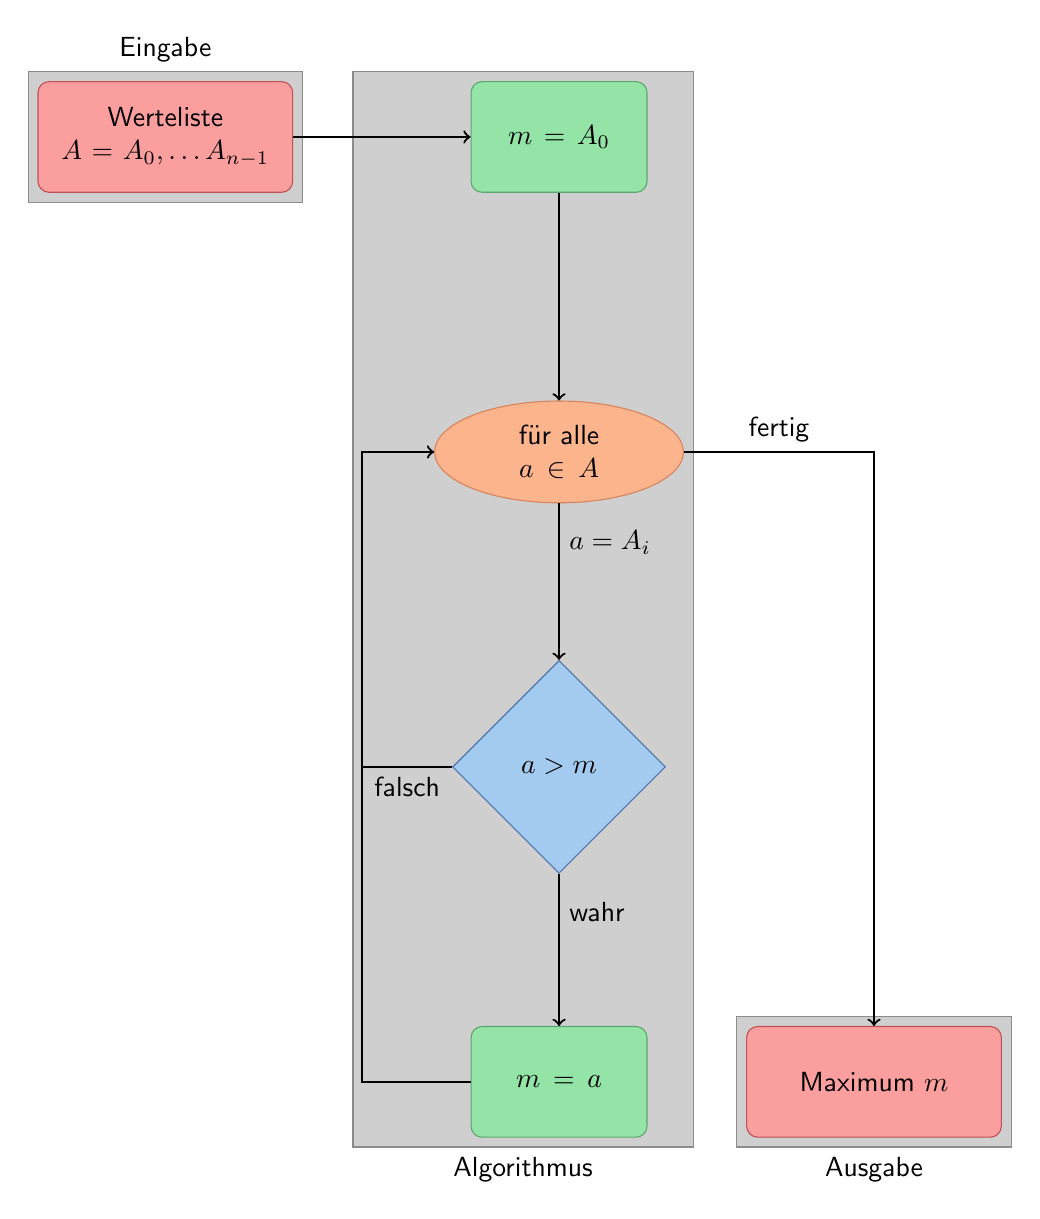
\begin{tikzpicture}[node distance = 4cm and 6cm, auto]

	\definecolor{my_blue}{RGB}{80,116,172}
\definecolor{my_blue_dark}{RGB}{3,33,122}
\definecolor{my_blue_light}{RGB}{163,203,240}

\definecolor{my_orange}{RGB}{217,132,92}
\definecolor{my_orange_dark}{RGB}{173,64,35}
\definecolor{my_orange_light}{RGB}{251,180,139}

\definecolor{my_green}{RGB}{91,166,108}
\definecolor{my_green_dark}{RGB}{32,112,42}
\definecolor{my_green_light}{RGB}{148,228,167}

\definecolor{my_red}{RGB}{192,80,86}
\definecolor{my_red_dark}{RGB}{136,11,17}	
\definecolor{my_red_light}{RGB}{251,159,158}	

\definecolor{my_violet}{RGB}{128,116,174}
\definecolor{my_violet_dark}{RGB}{87,34,108}	
\definecolor{my_violet_light}{RGB}{207,189,250}

\definecolor{my_brown}{RGB}{145,120,100}
\definecolor{my_brown_dark}{RGB}{159,187,159}	
\definecolor{my_brown_light}{RGB}{87,47,21}

\definecolor{my_pink}{RGB}{215,141,192}
\definecolor{my_pink_dark}{RGB}{247,177,225}	
\definecolor{my_pink_light}{RGB}{158,56,127}

\definecolor{my_gray}{RGB}{140,140,140}
\definecolor{my_gray_dark}{RGB}{60,60,60}
\definecolor{my_gray_light}{RGB}{207,207,207}

\definecolor{my_yellow}{RGB}{203,184,125}
\definecolor{my_yellow_dark}{RGB}{255,253,175}	
\definecolor{my_yellow_light}{RGB}{182,132,48}

\definecolor{my_turkis}{RGB}{106,181,202}
\definecolor{my_turkis_dark}{RGB}{189,242,240}	
\definecolor{my_turkis_light}{RGB}{20,99,114}

\tikzstyle{decision} = [diamond, draw, draw=my_blue, fill=my_blue_light, text width=2.5cm, text badly centered, inner sep=0pt]
\tikzstyle{block} = [rectangle, draw=my_green, fill=my_green_light, text width=2cm, text centered, rounded corners, minimum height=4em]
\tikzstyle{blockio} = [rectangle, draw=my_red, fill=my_red_light, text width=3cm, text centered, rounded corners, minimum height=4em]
\tikzstyle{cloud} = [text centered, ellipse, draw=my_orange, fill=my_orange_light, text width=2cm, minimum height=3em]
\tikzstyle{line} = [draw, thick]

\tikzstyle{back_box} = [draw=my_gray, fill=my_gray_light, behind path]

	\node [blockio] (eingabe) {Werteliste\\$A=A_0, \dots A_{n-1}$};
  
	\node [block, right of=eingabe, node distance=5cm] (init) {$m=A_0$};
  
	\node [cloud, below of=init] (loop) {für alle $a\in A$};
	\node [decision, below of=loop] (check_max) {$a>m$};
	\node [block, below of=check_max] (set_max) {$m=a$};

	\node [blockio, right of=set_max] (ausgabe) {Maximum $m$};
	\node [coordinate, left of=check_max, node distance=2.5cm] (c1) {};

	\begin{scope}[on background layer]
		\node[back_box, fit=(init) (loop) (check_max) (set_max) (c1), label=below:Algorithmus] (algo_box) {};
		\node[back_box, fit=(eingabe), label=above:Eingabe] (input) {};
		\node[back_box, fit=(ausgabe), label=below:Ausgabe] (output) {};
	\end{scope}

	\path [line, ->] (eingabe) -- (init);
	\path [line, ->] (init) -- (loop);  
	\path [line, ->] (loop) -| node [near start] {fertig}  (ausgabe);  
	\path [line, ->] (loop) -- node [near start] {$a=A_i$} (check_max);
	\path [line, ->] (check_max) -- node [near start] {wahr} (set_max);     
	\draw [line] (check_max) -- node [midway] {falsch} (c1);
	\draw [line] (set_max) -| (c1);
	\draw [line, ->] (c1) |- (loop);
	

\end{tikzpicture}
\end{document}
